% Auto-generated editable source. Edit freely in VS Code.
% Parallel source; the live site is pages/proj-verify-agents.html.
\documentclass[11pt]{article}
\usepackage[margin=1in]{geometry}
\usepackage{graphicx}
\usepackage{hyperref}
\usepackage{enumitem}
\usepackage{xcolor}
\definecolor{aidred}{HTML}{A8324A}
\definecolor{aidpink}{HTML}{CF4D87}
\hypersetup{colorlinks=true,linkcolor=aidpink,urlcolor=aidpink,citecolor=aidpink}
\newcommand{\finding}[2]{\par\medskip\noindent{\color{aidred}\textbf{Finding #1.}}~#2\par\medskip}

\title{When the Verifier Is Wrong}
\author{Saanvi S. Subramanian \\ \small California Institute of Technology}
\date{\small poster, Verify-Agents @ NeurIPS 2026 \quad\textbullet\quad sole author}
\begin{document}
\maketitle

\begin{abstract}
\noindent A closed-loop protein-design agent picks candidates from a pool of thousands, and a trust gate decides whether to delegate that ranking to a supplied scorer by checking the scorer's AUROC against the outcomes collected so far. The gate never verifies that the supplied scorer is parameter-free, which is the vulnerability. Across 41 deep mutational scans of 1{,}800 to 7{,}900 candidates each, plus five published multi-round campaigns from ProteinGym, FLIP and PETML, a scorer that memorizes the observed outcomes clears the gate at AUROC 0.991 and passes every trial while adding nothing. Forward validation closes that hole but cannot see a pool-side attack that leaves measured scores untouched. A probe catches the pool-side attack yet recovers only about 10\% of the lost value, because catching an attack and replacing it are different problems.
\end{abstract}

\section*{How the gate breaks}
The agent ranks a pool of unmeasured candidates with a supplied scorer, tests a batch, and feeds the outcomes back. Before trusting the scorer, a gate scores it on the outcomes collected so far. The attacks below are ordered by the defense each one defeats.

\begin{description}[leftmargin=1.2em]
  \item[The leakage attack.] A scorer that memorizes the observed outcomes and outputs noise everywhere else. Across 4{,}920 trials, a fully leaked scorer reaches gate AUROC 0.991 and passes 100\% of trials, against 0.663 and 77.2\% for a truthful zero-shot scorer. It ranks above the useful scorer and performs at random on the unmeasured pool, costing about 1.05 good candidates per batch. Even 25\% leakage passes 77\% of the time.
  \item[Forward validation, and why it is not enough.] Score the scorer only on measurements collected after it was supplied. Acquisition order creates the holdout, so the gate never inspects the scorer's implementation. The truthful scorer holds at 0.687 and 79.5\% while the fully leaked scorer falls to 0.495 and 34.8\%, the finite-sample false-pass floor rather than residual signal.
  \item[The pool-side attack forward validation cannot see.] Leave every measured candidate untouched and corrupt only the unmeasured pool. Because the measured scores are unchanged, both gates return identical statistics to the truthful scorer by construction, 0.663 and 0.676. The selections lose 1.24 good candidates per batch.
  \item[Top-pick probing, and probe-aware evasion.] Measure a prefix of the scorer's own top picks before committing the batch. A 25\% probe detects 99.2\% of naive pool-side attacks while costing the truthful scorer 4.4\% of its yield. An attacker who baits the top of the ranking to match the probe drops detection to 45.9\%, and to 39.6\% at a 50\% probe.
\end{description}

\finding{1}{A trust gate that evaluates a supplied scorer in sample certifies a scorer that has memorized the evaluation outcomes. It ranks that scorer above a truthful one at AUROC 0.991 against 0.663, passes it in every trial, and the agent loses about 1.05 good candidates per batch for following it.}

\finding{2}{Forward validation closes the leakage surface and nothing else. An attacker restricted to the unmeasured pool produces gate statistics identical to the truthful scorer by construction and costs 1.24 good candidates per batch. Detecting it requires spending experimental budget on candidates the scorer currently recommends.}

\begin{figure}[h]\centering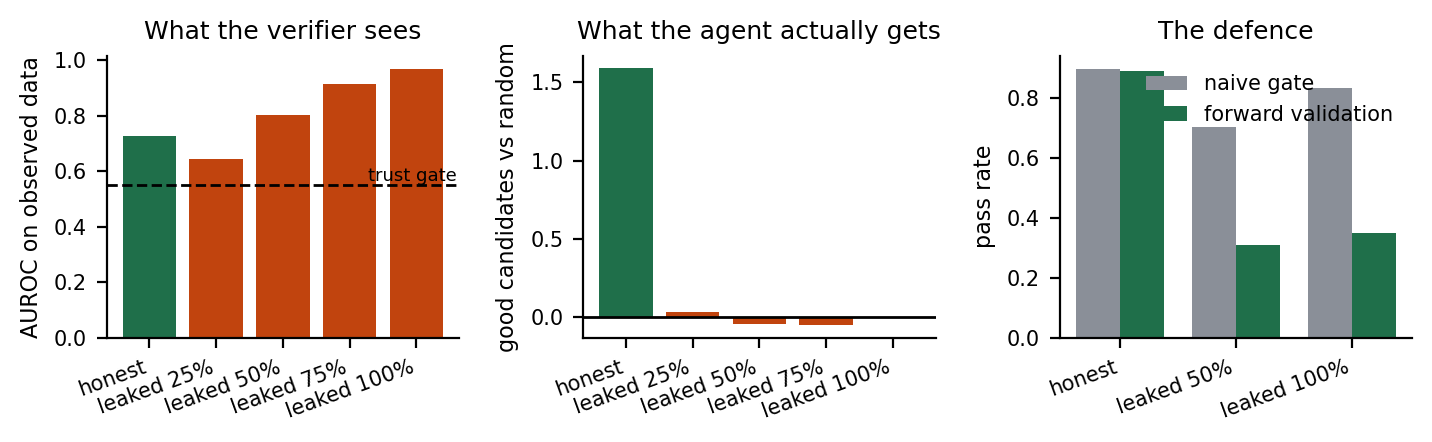
\includegraphics[width=\textwidth]{../../assets/images/projects/agentevals/verifier-attack.png}
\caption*{\textcolor{aidred}{\textbf{Figure 1. The gate rewards the wrong signal.}} Left, the gate's score rises with leakage; at a 25\% leak it already sits just below the truthful scorer. Center, selection value, where only the truthful scorer helps. Right, forward validation holds the truthful scorer's value while pushing the leaked scorers to chance.}\end{figure}

\begin{figure}[h]\centering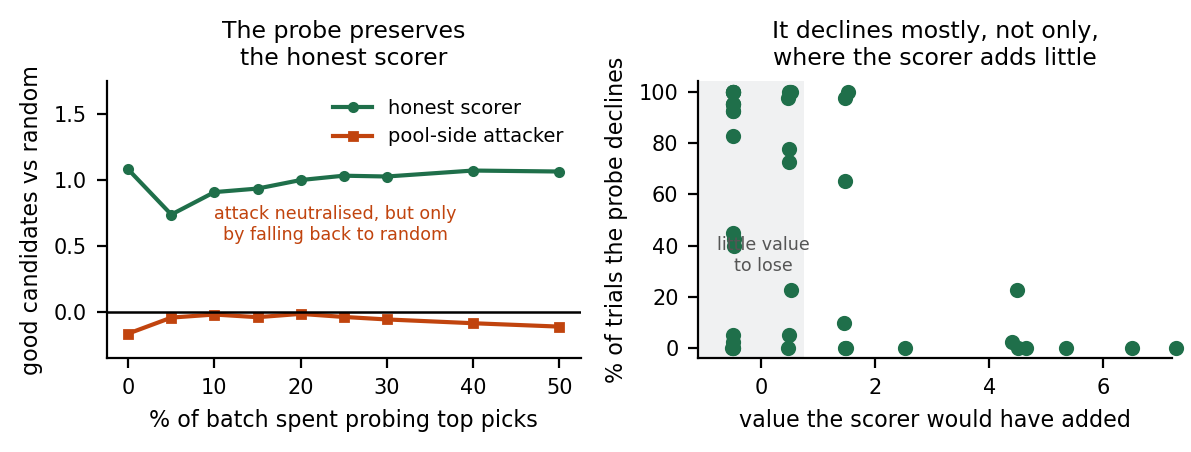
\includegraphics[width=\textwidth]{../../assets/images/projects/agentevals/verifier-probe.png}
\caption*{\textcolor{aidred}{\textbf{Figure 2. Top-pick probing across all 41 scans.}} Left, probing keeps most of the truthful scorer's value while driving the pool-side attacker to random. Right, the probe rejects the truthful scorer on 48\% of trials, but those are trials where it would have captured 0.142 good candidates against 1.943 on the trials it accepts.}\end{figure}

\finding{3}{Detection is not recovery. The probe catches nearly every naive pool-side attack but recovers only about 10\% of the lost value when the fallback is random selection, moving the agent from $-0.162$ to $-0.036$ where the truthful scorer would have given $+1.082$. An in-house ridge model trained on the campaign's own 48 measurements recovers 17\% at a 25\% probe and 28\% at a 50\% probe, and overtakes the supplied scorer after roughly 115 measurements, reaching $+1.745$ against $+0.741$ at 384.}

\begin{figure}[h]\centering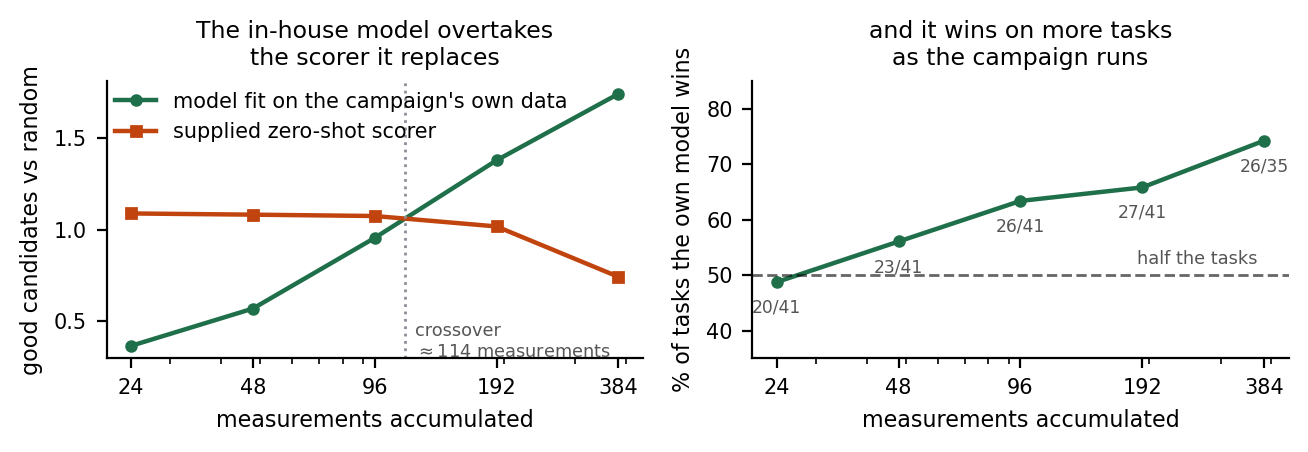
\includegraphics[width=\textwidth]{../../assets/images/projects/agentevals/verifier-crossover.png}
\caption*{\textcolor{aidred}{\textbf{Figure 3. The supplied scorer loses its advantage as data accumulate.}} Left, good candidates per batch for the in-house and supplied scorers as the campaign grows; right, the fraction of tasks where the in-house model wins. The eligible task set shrinks from 41 to 35 at 384 measurements, so this is a within-task comparison at each size.}\end{figure}

\paragraph{Why detection without a fallback fails.} If being caught sends the agent to random selection, and the attacker's goal was already to reduce the agent to random, detection imposes almost no cost on the attacker. A verifier needs a fallback that preserves value, which means an independent source of capability outside the compromised scorer's control. Verification can tell you when you need that. It cannot supply it.

\section*{Limitations}
The evaluation is offline and counterfactual on pools that earlier experimental choices already selected, so differences between policies are interpretable and absolute performance is not a population estimate. The policy-transfer experiment covers six non-LLM policy classes and shows that damage follows the fraction of action selection delegated to the compromised scorer, with the gate reading 0.6632 under both conditions and changing its decision in 0 of 1{,}640 trials. Transfer to an LLM-driven research agent is untested, and the mapping is conceptual.

\end{document}
